% Options for packages loaded elsewhere
% Options for packages loaded elsewhere
\PassOptionsToPackage{unicode}{hyperref}
\PassOptionsToPackage{hyphens}{url}
%
\documentclass[
  ignorenonframetext,
  aspectratio=169,
  spanish,
]{beamer}
\newif\ifbibliography
\usepackage{pgfpages}
\setbeamertemplate{caption}[numbered]
\setbeamertemplate{caption label separator}{: }
\setbeamercolor{caption name}{fg=normal text.fg}
\beamertemplatenavigationsymbolshorizontal
% remove section numbering
\setbeamertemplate{part page}{
  \centering
  \begin{beamercolorbox}[sep=16pt,center]{part title}
    \usebeamerfont{part title}\insertpart\par
  \end{beamercolorbox}
}
\setbeamertemplate{section page}{
  \centering
  \begin{beamercolorbox}[sep=12pt,center]{section title}
    \usebeamerfont{section title}\insertsection\par
  \end{beamercolorbox}
}
\setbeamertemplate{subsection page}{
  \centering
  \begin{beamercolorbox}[sep=8pt,center]{subsection title}
    \usebeamerfont{subsection title}\insertsubsection\par
  \end{beamercolorbox}
}
% Prevent slide breaks in the middle of a paragraph
\widowpenalties 1 10000
\raggedbottom
\AtBeginPart{
  \frame{\partpage}
}
\AtBeginSection{
  \ifbibliography
  \else
    \frame{\sectionpage}
  \fi
}
\AtBeginSubsection{
  \frame{\subsectionpage}
}
\usepackage{iftex}
\ifPDFTeX
  \usepackage[T1]{fontenc}
  \usepackage[utf8]{inputenc}
  \usepackage{textcomp} % provide euro and other symbols
\else % if luatex or xetex
  \usepackage{unicode-math} % this also loads fontspec
  \defaultfontfeatures{Scale=MatchLowercase}
  \defaultfontfeatures[\rmfamily]{Ligatures=TeX,Scale=1}
\fi
\usepackage{lmodern}

\usetheme[]{default}
\usefonttheme[]{default}
\ifPDFTeX\else
  % xetex/luatex font selection
\fi
% Use upquote if available, for straight quotes in verbatim environments
\IfFileExists{upquote.sty}{\usepackage{upquote}}{}
\IfFileExists{microtype.sty}{% use microtype if available
  \usepackage[]{microtype}
  \UseMicrotypeSet[protrusion]{basicmath} % disable protrusion for tt fonts
}{}
\makeatletter
\@ifundefined{KOMAClassName}{% if non-KOMA class
  \IfFileExists{parskip.sty}{%
    \usepackage{parskip}
  }{% else
    \setlength{\parindent}{0pt}
    \setlength{\parskip}{6pt plus 2pt minus 1pt}}
}{% if KOMA class
  \KOMAoptions{parskip=half}}
\makeatother


\usepackage{longtable,booktabs,array}
\usepackage{calc} % for calculating minipage widths
\usepackage{caption}
% Make caption package work with longtable
\makeatletter
\def\fnum@table{\tablename~\thetable}
\makeatother
\usepackage{graphicx}
\makeatletter
\newsavebox\pandoc@box
\newcommand*\pandocbounded[1]{% scales image to fit in text height/width
  \sbox\pandoc@box{#1}%
  \Gscale@div\@tempa{\textheight}{\dimexpr\ht\pandoc@box+\dp\pandoc@box\relax}%
  \Gscale@div\@tempb{\linewidth}{\wd\pandoc@box}%
  \ifdim\@tempb\p@<\@tempa\p@\let\@tempa\@tempb\fi% select the smaller of both
  \ifdim\@tempa\p@<\p@\scalebox{\@tempa}{\usebox\pandoc@box}%
  \else\usebox{\pandoc@box}%
  \fi%
}
% Set default figure placement to htbp
\def\fps@figure{htbp}
\makeatother



\ifLuaTeX
\usepackage[bidi=basic]{babel}
\else
\usepackage[bidi=default]{babel}
\fi
% get rid of language-specific shorthands (see #6817):
\let\LanguageShortHands\languageshorthands
\def\languageshorthands#1{}


\setlength{\emergencystretch}{3em} % prevent overfull lines

\providecommand{\tightlist}{%
  \setlength{\itemsep}{0pt}\setlength{\parskip}{0pt}}



 


\setbeamertemplate{headline}{} % Elimina la cabecera del tema Madrid
\setbeamertemplate{section in head/foot}{} % Limpia la numeración de secciones
\renewcommand{\contentsname}{Índice}
\renewcommand{\refname}{Referencias}
\renewcommand{\figurename}{Figura}
\renewcommand{\tablename}{Tabla}
\logo{%
  \begin{tabular}{c}
    
\includegraphics[height=1.2cm]{EscudoU.png}
  \end{tabular}%
}
% --- CONFIGURACIÓN DE COLORES INSTITUCIONALES ---
\definecolor{UnicorGreen}{HTML}{024426}
\definecolor{UnicorText}{HTML}{F9F9F9}
\definecolor{UnicorWhite}{HTML}{FFFFFF}
\definecolor{UnicorGold}{HTML}{D1B061}

% Aplicación al fondo y texto general
\setbeamercolor{background canvas}{bg=UnicorGreen}
\setbeamercolor{normal text}{fg=UnicorText}

% Aplicación a títulos y cabeceras
%\setbeamercolor{title}{fg=UnicorWhite}
\setbeamercolor{frametitle}{fg=UnicorWhite}
\setbeamercolor{framesubtitle}{fg=UnicorWhite}

% Aplicación a viñetas y estructura
\setbeamercolor{structure}{fg=UnicorWhite}
\setbeamercolor{itemize item}{fg=UnicorWhite}
\setbeamercolor{itemize subitem}{fg=UnicorWhite}
\setbeamercolor{enumerate item}{fg=UnicorWhite}

% Forzar a LaTeX a repintar el texto general al iniciar el documento
\AtBeginDocument{\usebeamercolor[fg]{normal text}}

% Aplicación a hipervínculos
\hypersetup{colorlinks=true, urlcolor=UnicorGold, linkcolor=UnicorWhite}

% --- ACTIVAR ESTILO DE BLOQUES Y SOMBRAS (ESTILO MADRID) ---
\useinnertheme[shadow=true]{rounded}

% --- COLORES DEL RECUADRO DEL TÍTULO PRINCIPAL ---
% Fondo dorado con texto verde
\setbeamercolor{title}{bg=UnicorGold, fg=UnicorGreen}
\setbeamercolor{frametitle}{fg=UnicorWhite} % Mantiene el título de las diapositivas normal
\setbeamercolor{framesubtitle}{fg=UnicorWhite}

% --- COLORES PARA TEOREMAS, DEFINICIONES Y BLOQUES ---
% Título del bloque (Fondo dorado, texto verde)
\setbeamercolor{block title}{bg=UnicorGold, fg=UnicorGreen}
% Cuerpo del bloque (Fondo blanco, texto verde)
\setbeamercolor{block body}{bg=UnicorWhite, fg=UnicorGreen}

\AtBeginDocument{
  \author{%
    \begin{tabular}{c}
      Mario A. Morales Rivera \\
      \footnotesize \texttt{mamorales@correo.unicordoba.edu.co} \\
      \footnotesize Universidad de Córdoba
    \end{tabular}
  }
  \institute{}
}
% --- LIMPIAR DIAPOSITIVAS DE SECCIÓN (ELIMINAR "SECTION X") ---
\setbeamertemplate{section page}{
  \begin{center}
    \begin{beamercolorbox}[sep=12pt,center,rounded=true,shadow=true]{title}
      \usebeamerfont{title}\insertsection\par
    \end{beamercolorbox}
  \end{center}
}
\makeatletter
\@ifpackageloaded{tcolorbox}{}{\usepackage[skins,breakable]{tcolorbox}}
\@ifpackageloaded{fontawesome5}{}{\usepackage{fontawesome5}}
\definecolor{quarto-callout-color}{HTML}{909090}
\definecolor{quarto-callout-note-color}{HTML}{0758E5}
\definecolor{quarto-callout-important-color}{HTML}{CC1914}
\definecolor{quarto-callout-warning-color}{HTML}{EB9113}
\definecolor{quarto-callout-tip-color}{HTML}{00A047}
\definecolor{quarto-callout-caution-color}{HTML}{FC5300}
\definecolor{quarto-callout-color-frame}{HTML}{acacac}
\definecolor{quarto-callout-note-color-frame}{HTML}{4582ec}
\definecolor{quarto-callout-important-color-frame}{HTML}{d9534f}
\definecolor{quarto-callout-warning-color-frame}{HTML}{f0ad4e}
\definecolor{quarto-callout-tip-color-frame}{HTML}{02b875}
\definecolor{quarto-callout-caution-color-frame}{HTML}{fd7e14}
\makeatother
\makeatletter
\@ifpackageloaded{caption}{}{\usepackage{caption}}
\AtBeginDocument{%
\ifdefined\contentsname
  \renewcommand*\contentsname{Tabla de contenidos}
\else
  \newcommand\contentsname{Tabla de contenidos}
\fi
\ifdefined\listfigurename
  \renewcommand*\listfigurename{Listado de Figuras}
\else
  \newcommand\listfigurename{Listado de Figuras}
\fi
\ifdefined\listtablename
  \renewcommand*\listtablename{Listado de Tablas}
\else
  \newcommand\listtablename{Listado de Tablas}
\fi
\ifdefined\figurename
  \renewcommand*\figurename{Figura}
\else
  \newcommand\figurename{Figura}
\fi
\ifdefined\tablename
  \renewcommand*\tablename{Tabla}
\else
  \newcommand\tablename{Tabla}
\fi
}
\@ifpackageloaded{float}{}{\usepackage{float}}
\floatstyle{ruled}
\@ifundefined{c@chapter}{\newfloat{codelisting}{h}{lop}}{\newfloat{codelisting}{h}{lop}[chapter]}
\floatname{codelisting}{Listado}
\newcommand*\listoflistings{\listof{codelisting}{Listado de Listados}}
\makeatother
\makeatletter
\makeatother
\makeatletter
\@ifpackageloaded{caption}{}{\usepackage{caption}}
\@ifpackageloaded{subcaption}{}{\usepackage{subcaption}}
\makeatother

\usepackage{bookmark}
\IfFileExists{xurl.sty}{\usepackage{xurl}}{} % add URL line breaks if available
\urlstyle{same}
\hypersetup{
  pdftitle={Cálculos con variables discretas},
  pdfauthor={Mario Morales},
  pdflang={es},
  hidelinks,
  pdfcreator={LaTeX via pandoc}}


\title{Cálculos con variables discretas}
\subtitle{Probabilidades puntuales, acumuladas, quantiles y generación
de numeros aleatorios}
\author{Mario Morales}
\date{14/10/2026}

\begin{document}
\frame{\titlepage}

\renewcommand*\contentsname{Tabla de contenidos}
\begin{frame}[allowframebreaks]
  \frametitle{Tabla de contenidos}
  \setcounter{tocdepth}{3}
  \tableofcontents
\end{frame}
\setcounter{tocdepth}{3}
\tableofcontents
}

\section{Introducción}\label{introducciuxf3n}

\begin{frame}{Introducción}
\phantomsection\label{introducciuxf3n-1}
Estudiamos en esta clase los modelos de probabilidad asociados a las
variables aleatorias discretas de uso frecuente. Definimos el modelo de
Bernoulli, binomial, geométrico, binomial negativo, hipergeométrico y de
Poisson, estableciendo los supuestos que deben cumplir los experimentos
aleatorios que dan lugar a ellos. Al finalizar la clase el estudiante
estará en capacidad de usar R para llevar a cabo el cálculo de
probabilidades puntuales y acumuladas, cuantiles y generar datos pseudo
aleatorios usando estos modelos.
\end{frame}

\section{Funciones para modelos discretos con
R}\label{funciones-para-modelos-discretos-con-r}

\begin{frame}[fragile]{Funciones \texttt{d}: \emph{density}}
\phantomsection\label{funciones-d-density}
\begin{itemize}
\tightlist
\item
  función \texttt{d}: \emph{density} permite el calculo de
  probabilidades puntuales, es decir, con esta función se evalúa la
  función de probabilidad.
\end{itemize}

Por ejemplo, en el caso de la distribución binomial,
\texttt{dbinom(x,n,pi)} evalúa la función
\[\binom{n}{x}\pi^{x}(1-\pi)^{(n-x)}\]
\end{frame}

\begin{frame}[fragile]{Funciones \texttt{p}: \emph{probability}}
\phantomsection\label{funciones-p-probability}
\begin{itemize}
\tightlist
\item
  función \texttt{p}: para evaluar la función de distribución del modelo
  definido.
\end{itemize}

Por ejemplo, en el caso binomial evalúa
\[\sum_{k=0}^x\binom{n}{k}\pi^{k}(1-\pi)^{(n-k)}\]
\end{frame}

\begin{frame}[fragile]{Funciones \texttt{r}: \emph{random}}
\phantomsection\label{funciones-r-random}
Las funciones \texttt{r}: \emph{random} se usan para generar (simular)
datos pseudo aleatorios que siguen la distribución del modelo.
\end{frame}

\begin{frame}[fragile]{Funciones \texttt{q}: \emph{quantile}}
\phantomsection\label{funciones-q-quantile}
\begin{itemize}
\item
  Las funciones \texttt{q}: \emph{quantile} se usan para el cálculo de
  percentiles de la distribución.
\item
  Este método implementa la función inversa de la \texttt{cdf}.
\end{itemize}

\begin{tcolorbox}[enhanced jigsaw, toprule=.15mm, bottomrule=.15mm, left=2mm, bottomtitle=1mm, leftrule=.75mm, opacitybacktitle=0.6, breakable, titlerule=0mm, title=\textcolor{quarto-callout-important-color}{\faExclamation}\hspace{0.5em}{Importante}, rightrule=.15mm, colback=white, toptitle=1mm, coltitle=black, colbacktitle=quarto-callout-important-color!10!white, arc=.35mm, opacityback=0, colframe=quarto-callout-important-color-frame]

Dada una probabilidad \(p\), la función \texttt{q} regresa el valor mas
pequeño \(x\) tal que \(P(X\leq x )\ge p\).

\end{tcolorbox}
\end{frame}

\begin{frame}[fragile]{Modelo Binomial (I)}
\phantomsection\label{modelo-binomial-i}
Un experimento aleatorio que consiste de

\begin{itemize}
\item
  \(n\) repeticiones independientes de experimentos de Bernoulli,
\item
  la probabilidad de éxito, \(\pi\), de cada experimento permanece
  constante, se conoce como un experimento \texttt{Binomial}.
\item
  la variable de interés es el número de éxitos en los \(n\) ensayos.
\end{itemize}
\end{frame}

\begin{frame}{Ejemplos de experimentos Binomiales}
\phantomsection\label{ejemplos-de-experimentos-binomiales}
\begin{itemize}
\tightlist
\item
  Lanzar tres monedas y contar el número de sellos, que consideraremos
  éxitos.
\item
  Examinar 20 ratas de laboratorio después de someterlas a cierta dieta
  y observar si desarrollaron cáncer de estómago (éxito).
\item
  Se someten insectos a cierta concentración de un veneno durante 30
  minutos y al final, para cada uno, se registra si sobrevive (fracaso)
  o no (éxito).
\item
  Se eligen 100 personas al azar del censo electoral y se registra, para
  cada uno si votará (éxito) o no (fracaso) por cierto candidato a un
  cargo de elección popular.
\end{itemize}
\end{frame}

\begin{frame}{Modelo Binomial (II)}
\phantomsection\label{modelo-binomial-ii}
En cada uno de los experimentos anteriores, nos interesa registrar el
número de éxitos en los \(n\) ensayos de Bernoulli. Sea \(X\) la función
que toma cada punto del espacio muestral del experimento y le hace
corresponder el número de éxitos, necesitamos una fórmula que nos
permita calcular las probabilidades asociadas a cada posible valor que
toma la función.
\end{frame}

\begin{frame}{Modelo Binomial (III)}
\phantomsection\label{modelo-binomial-iii}
Suponga que se lanzan tres monedas (o una moneda tres veces) y
registramos el resultado en el lado que queda hacia arriba (Cara o
Sello). Consideremos la función (variable aleatoria) que asigna a cada
punto del espacio muestral el número de sellos.
\end{frame}

\begin{frame}{}
\phantomsection\label{section}
\begin{figure}[H]

{\centering \pandocbounded{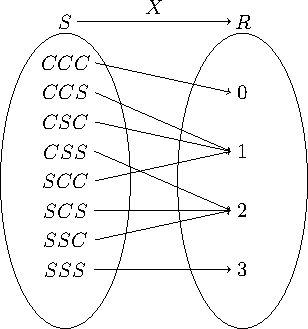
\includegraphics[keepaspectratio]{VADiscretas_files/figure-beamer/unnamed-chunk-1-1.pdf}}

}

\caption{Mapeo de los resultados a la variable aleatoria X}

\end{figure}%
\end{frame}

\begin{frame}{Modelo Binomial (III)}
\phantomsection\label{modelo-binomial-iii-1}
\begin{itemize}
\item
  En la figura se muestra el diagrama de flechas de la función, \(SSC\)
  significa que la primera moneda resultó cara, la segunda y la tercera
  sello. Por la forma que se ha definido la función, \(X(SSC)\to 2\), ya
  que el punto tiene dos sellos.
\item
  Para calcular \(P(X=2)\) se tiene en cuenta que los ensayos son
  independientes, además, considerando \(S\) como éxito y \(C\) fracaso,
  con probabilidad \(\pi\) y \(1-\pi\) respectivamente, la probabilidad
  conjunta del resultado \(SSC\) es \[P(SSC)=P(S)P(S)P(C)=\pi^2(1-\pi)\]
\end{itemize}
\end{frame}

\begin{frame}{Modelo Binomial (IV)}
\phantomsection\label{modelo-binomial-iv}
\begin{itemize}
\tightlist
\item
  Por la definición dada en la sección anterior, debido a que hay tres
  puntos en \(S\) que se asignan a 2 por la función, entonces
  \[P(X=2)=P(\{CSS,SCS,SSC\})=3\pi^2(1-\pi)\] con un razonamiento
  similar se calculan las probabilidades de \(X=0\), \(X=1\) y \(X=3\)
  que se muestran en la tabla
\end{itemize}
\end{frame}

\begin{frame}{Modelo Binomial (V)}
\phantomsection\label{modelo-binomial-v}
\begin{itemize}
\item
  Supongamos que se lanzan \(n\) monedas y a cada punto del espacio
  muestral de este experimento hacemos corresponder el número de sellos
  en la cara superior, supongamos que se obtienen \(x\) sellos y \(n-x\)
  caras, con \(x=0,1,2,\ldots,n\).
\item
  Por el supuesto de independencia, sin importar la posición en que
  aparezcan los sellos y las caras la probabilidad de un punto con \(x\)
  sellos y \(n-x\) caras es \(\pi^x(1-\pi)^{n-x}\) y hay
  \(\tbinom{n}{x}\) formas de salir \(x\) sellos, por tanto
  \[P(X=x)=\binom{n}{x}\pi^x(1-\pi)^{n-x}\]
\end{itemize}
\end{frame}

\begin{frame}{Modelo Binomial (VI)}
\phantomsection\label{modelo-binomial-vi}
\begin{itemize}
\tightlist
\item
  En conclusión, si \(X\) es la variable aleatoria que cuenta el número
  de éxitos en \(n\) ensayos de Bernoulli, independientes, con
  probabilidad de éxito constante \(\pi\), su función de probabilidad
  esta dada por\\
  \[
  f_X(x)=P(X=x)=\begin{cases}
  \binom{n}{x}\pi^{x}(1-\pi)^{(n-x)} \text{ para } x=0,1,2,\ldots,  n  \\
  0 \text{ en cualquier otro }  x \in R 
  \end{cases}  
  \end{equation*} 
  La función de distribución de $X$ es 
  \begin{equation*} 
  F_X(x)=P(X\leq x)=
  \sum_{k=0}^x\binom{n}{k}\pi^{k}(1-\pi)^{(n-k)} 
  \]
\end{itemize}
\end{frame}




\end{document}
